\chapter{Metodologia}\label{metodologia}
% ---

% MARCELO 17/05: vamos transformar numa seção do capítulo anterior.
Para a realização do embasamento deste trabalho, foram utilizadas tanto a metodologia de pesquisa bibliográfica 
quanto a de pesquisa documental. A primeira foi essencial para o levantamento de metodologias já consolidadas e 
amplamente estudadas, como as que serão abordadas no referencial teórico e, a seguir, nesta seção. Já a segunda 
foi empregada para identificar diferentes aplicações correlatas e para a elaboração do referencial teórico, além 
de ter sido utilizada na análise de dados internos do CECLIMAR, conforme comentado na conforme comentado na 
\hyperref[chapter:intro]{Introdução} deste trabalho.
% MARCELO 13/05: remover a palavra grande. dispersos aonde?
% VITOR 20/05: OK palavra
Segundo \citeonline{gil2002elaborar}, a pesquisa bibliográfica é desenvolvida com base em materiais como livros 
e artigos científicos, ou seja, materiais já consolidados. Trata-se de uma pesquisa de grande importância, pois 
% MARCELO 13/05: remover a palavra muito.
% VITOR 20/05: OK
permite que os pesquisadores acessem diversos dados e informações dispersos que, individualmente, seriam 
trabalhosos e custosos de se coletar. Nesse tipo de pesquisa, entretanto, é necessário ter cuidado com citações 
de terceiros, que podem interpretar de forma equivocada algum dado ou informação originalmente levantados.

Ainda segundo o autor, a pesquisa documental se diferencia pela natureza das fontes de informação. Enquanto as 
pesquisas bibliográficas consistem essencialmente em um apanhado de contribuições de diversos autores sobre 
determinado assunto, a pesquisa documental ocorre por meio de materiais que ainda não receberam tratamento 
analítico ou que podem ser reelaborados, a depender dos objetos de pesquisa. As fontes da pesquisa documental 
são mais diversas e podem incluir conversas pessoais, entrevistas, documentos ou sites.
% MARCELO 13/05: colocar referência para Google Scholar
% VITOR 20/05: OK
A metodologia de pesquisa bibliográfica foi realizada através da plataforma \citeonline{google_scholar_2025}, publicações 
% MARCELO 13/05: colocar referência para SiBBr
% VITOR 20/05: OK
presentes no portal do \citeonline{sibbr2024}, Sistema de Informação 
sobre a Biodiversidade Brasileira, além de livros disponibilizados na biblioteca 
do Instituto Federal Campus Osório. Já a metodologia de pesquisa documental 
foi levantada a partir de arquivos internos, relatórios das Nações Unidas e conteúdos disponibilizados por 
desenvolvedores ou organizações que participaram do desenvolvimento das aplicações correlatas.

Após a fase de revisão bibliográfica se iniciou o desenvolvimento do sistema. Esta fase foi realizada a 
partir do levantamento de requisitos junto de profissionais do CECLIMAR e, os requisitos levantados foram 
cadastrados e refinados para desenvolvimento cíclico do sistema. Cada ciclo visou a entrega de um produto 
com incrementos de requisitos pré estabelecidos. Ao final de cada um dos ciclos de desenvolvimento o sistema 
foi disponibilizado para testes com servidores do CECLIMAR, os \textit{feedbacks} recebidos foram analisados, 
refinados e postos para desenvolvimento no ciclo seguinte. Um ponto de atenção no desenvolvimento desse 
sistema é que, por se tratar de um sistema de ciência cidadã, deve estar adequado com a LGPD para que possa 
% MARCELO 13/05: colocar referência para PlayStore
% VITOR 20/05: OK
ser publicado na \citeonline{playstore2024} para o uso da sociedade.

% ---
\section{Metodologia de desenvolvimento de \textit{software}}\label{sec:metodologia-desenv-software}
% ---
% MARCELO 13/05: colocar referências aqui para Kanban e Jira
% VITOR 20/05: OK
Para o desenvolvimento deste projeto foi escolhida uma abordagem de metodologia ágil relacionada 
ao ciclo iterativo incremental \cite{pressman2011engenharia}. Utilizando o \textit{Kanban} como 
método de gestão de fluxo de trabalho \cite{ohno1988toyota}, a fim de melhorar a eficiência e qualidade do produto 
final a partir da visualização das tarefas. A ferramenta escolhida para realizar este 
gerenciamento foi o Jira \cite{atlassian_jira_2025}.

Segundo \citeonline{pressman2011engenharia}, os ciclos de desenvolvimento incremental podem ser 
divididos em 5 principais etapas: comunicação, planejamento, modelagem (análise e projeto), construção 
(codificação e testes) e emprego (entrega, \textit{feedback}). As etapas por ele descritas foram 
aplicadas neste projeto.
% MARCELO 13/05: trocar para o passado
% VITOR 20/05: OK
A comunicação foi marcada por reuniões agendadas com os profissionais do CECLIMAR para definição de
 escopo e levantamento de requisitos do sistema. O planejamento foi a análise, o refinamento e as 
 definições de quais funcionalidades foram desenvolvidas em cada ciclo. Durante a modelagem foi 
 realizada a prototipação e análise dos pontos levantados na etapa anterior. A construção foi o 
 momento onde a codificação e os testes da aplicação foram o foco de atuação. E, por fim, durante 
 o emprego o sistema 
 foi disponibilizado para os profissionais do CECLIMAR e uma 
 quantidade menor de usuários que contribuiram com 
 testes e retornos de \textit{feedback} para análise. Essas informações coletadas 
 foram catalogadas e inseridas no \textit{Backlog} 
 para serem puxados em um ciclo posterior.

%  é necessária uma nota de rodape para explicar o que é o MVP??
% MARCELO 13/05: por enquanto vamos deixar de fora. se necessário vamos colocar no referencial teorico
O uso desta metodologia tem o objetivo de realizar uma primeira entrega que possa ser considerada um 
Mínimo Produto Viável (\textit{MVP}) atendendo aos requisitos básicos propostos inicialmente, mesmo que ainda 
se note a ausência de funcionalidades complementares. Esse \textit{MVP} se tornará então a base de avaliação que 
permitirá identificar necessidades adicionais e ajustes necessários. Com base nessa análise, é planejado 
o próximo incremento, ajustando a primeira entrega e adicionando novas funcionalidades conforme as necessidades.

Para o desenvolvimento deste projeto, foi utilizado um fluxo de trabalho no \textit{Jira} para desenvolvimento de \textit{software} visando 
auxiliar no processo e manter a visibilidade das tarefas de ponta a ponta. Para o \textit{workflow} principal, 
foi montado um esquema com \textit{Backlog}, Refinamento, Em desenvolvimento, Aguardando teste, Em teste, 
Correção de \textit{bugs} e \textit{Done} (Figura~\ref{fig:fluxoJira}).

\begin{figure}[htb]
    \centering
    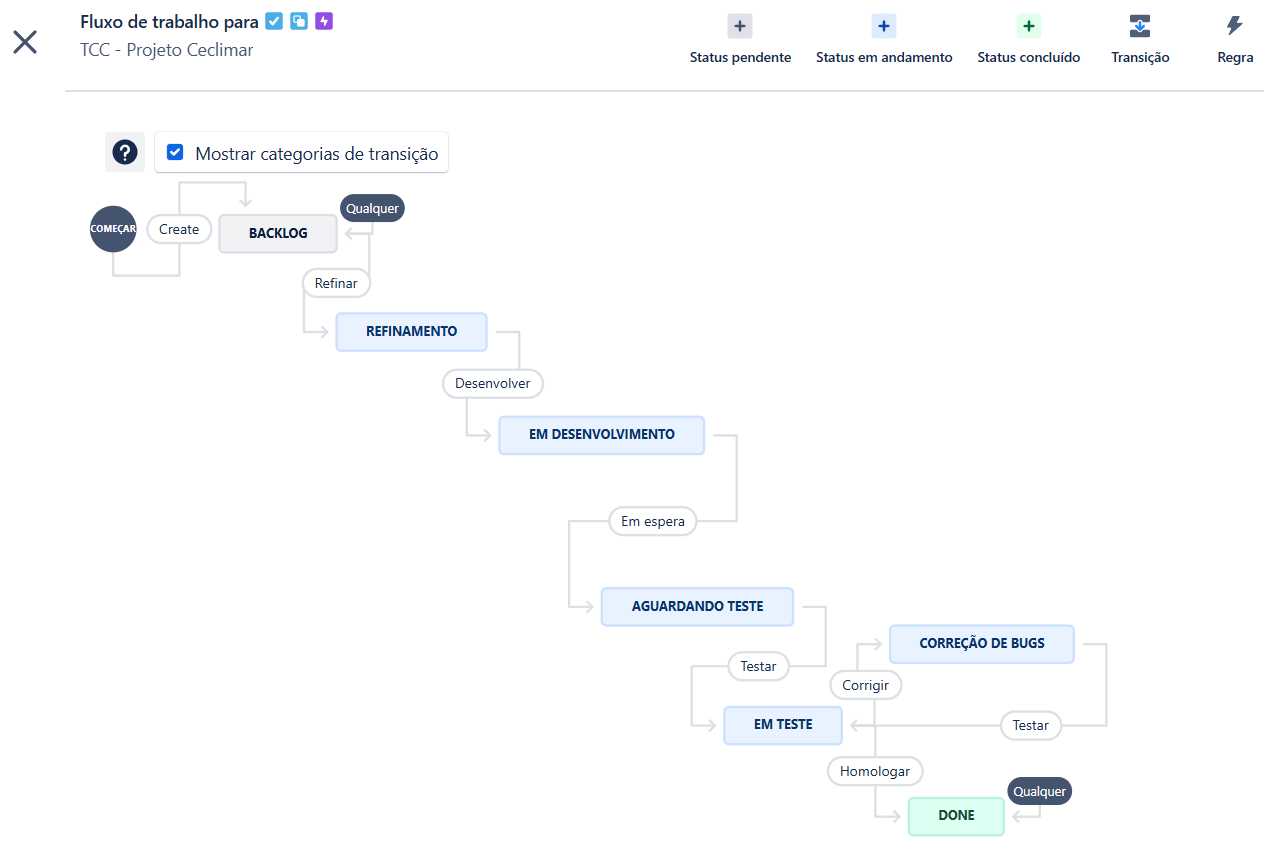
\includegraphics[width=0.8\textwidth]{imagens/fluxoJira.png}
    \caption{Fluxo de trabalho do \textit{Jira} gerado para o desenvolvimento do projeto.}
    \legend{Fonte: Autor}
    \label{fig:fluxoJira}
\end{figure} 

O \textit{Backlog} é a coluna onde todas as tarefas, \textit{user stories} e \textit{bugs} serão inicialmente 
posicionados. Nesta etapa, as tarefas serão priorizadas antes de andarem para o próximo estágio.

No Refinamento, as tarefas puxadas do \textit{Backlog} são detalhadas para um desenvolvimento 
mais assertivo. São refinados critérios de aceitação, estimativas de tempo e algum débito técnico.

As tarefas que estiverem em desenvolvimento são as que tiveram, efetivamente, o seu 
desenvolvimento iniciado. Assim que o desenvolvimento estiver finalizado, as tarefas 
serão transferidas para aguardando teste, onde ficarão até serem puxadas para testes 
mais detalhados.

No estágio de teste, os critérios de aceite e a presença de \textit{bugs} serão 
testados com o intuito de manter a qualidade do produto final. As tarefas que tiverem 
\textit{bugs} ou divergências de regras de negócio identificadas serão movidas para a coluna 
Correção de \textit{bugs} para que sejam corrigidas.

E, por último, após a homologação das tarefas nas etapas anteriores as tarefas 
são movidas para \textit{Done} que indicará sua finalização.

\section{Evolução Temporal do Projeto}\label{cronograma}
% MARCELO 17/05: UNIR COM A SEÇÃO DO CAPÍTULO ANTERIOR.
% VITOR 20/05: OK
% VITOR 07/06: o que acha desse titulo?
A Tabela ~\ref{tab:cronograma} representa a trajetória de 
desenvolvimento do projeto ao longo de 16 meses, bem como as divergências e 
replanejamentos que foram realizados no decorrer do tempo. O trabalho teve seu 
início no dia 28 de março de 2024, com a realização de uma reunião de definição 
de escopo junto do orientador Marcelo Paravisi. No dia 1º de abril, deu-se 
continuidade com a definição do tema, em uma reunião externa com um membro do 
CECLIMAR. Essa etapa foi fundamental para delimitar o foco do trabalho e aprofundar 
a compreensão das dificuldades, necessidades, oportunidades e pontos críticos do projeto

Os meses seguintes, de maio a julho de 2024, foram dedicados à revisão bibliográfica 
e à definição metodológica. A definição metodológica se deu durante o mês de maio 
tendo início no dia 06, enquanto a parte de revisão bibliográfica se iniciou no 
dia 05 do mesmo mês e foi finalizada no final de julho. 

O levantamento de requisitos e regras de negócio se deu a partir do dia 10 de 
maio e se estendeu até o final de agosto para que os alinhamentos de definições 
com a equipe do CECLIMAR fossem mais abertos e constantes. É importante ressaltar 
que durante o desenvolvimento houve mudanças de funcionalidades e ajustes de regras 
de negócio durante o período de testes que fizeram com que fosse necessário 
revisitar esse tópico. 

Esse período inicial de estruturação se mostrou essencial para assegurar uma base 
sólida para iniciar o desenvolvimento. A parte de desenvolvimento técnica se 
iniciou com a organização da implementação do sistema no dia 20 de maio de 2024 
e, com base nisso, se iniciou a codificação do aplicativo no dia 1º de julho do mesmo ano. 

Inicialmente, o desenvolvimento tinha um planejamento de conclusão para o final 
de outubro, porém, embora as atividades tenham progredido conforme o cronograma, 
em uma reunião com o orientador do projeto foi decido realizar uma alteração no 
cronograma adicionando uma etapa de testes disponibilizando a aplicação com 
testadores tanto do projeto parceiro, como terceiros que contribuíram para que 
a aplicação adquirisse uma maturidade maior. Com isso, o prazo final de codificação 
foi replanejado para o início de maio de 2025 (Tabela ~\ref{tab:cronograma}).

A parte de redação da parte escrita do trabalho de conclusão foi iniciada 
no mês de junho para obter uma documentação mais precisa 
do processo e estava planejada para ser concluída até o final de novembro 
de 2024, porém, também foi afetada pelo replanejamento. Em vermelho na 
Tabela ~\ref{tab:cronograma} podemos ver que esta etapa foi realizada dentro 
do prazo previsto até o mes de outubro, porém em novembro foi adiada para maio 
e junho para priorizar a conclusão da codificação e o aprimoramento da qualidade 
da aplicação.
O desenvolvimento continuou sendo a atividade central até maio de 2025, acompanhado 
de execuções constantes de testes. No mês de maio de 2025 a redação do trabalho 
retornou e se estendeu, junto da revisão textual, até o final de junho para ser 
entregue dentro da data máxima de 26 de junho. A apresentação para a banca até o 
momento havia sido definida, porém tem prazo máximo de 11 de julho de 2025.

Esse cronograma evidencia o fluxo de trabalho realizado desde o início do 
planejamento do projeto, bem como as alterações ocorridas durante seu desenvolvimento. 
Para a elaboração desse material, foi fundamental que os períodos de escrita e codificação 
estivessem bem alinhados, permitindo traçar e documentar, com maior precisão, a linha do 
tempo apresentada, desde o início até a entrega final planejada.

%VITOR 20/05: a tabela realmente ficou bem representativa? 
\begin{table}[ht]
\centering
\renewcommand{\arraystretch}{1.5}
\setlength{\tabcolsep}{4pt}
\resizebox{\textwidth}{!}{
\begin{tabular}{|>{\bfseries}l|*{11}{>{\centering\arraybackslash}p{1.6cm}|}}
\hline
\rowcolor{gray!20}
Meses & \rotatebox{90}{Reunião def. de escopo} & \rotatebox{90}{Definição de tema} & \rotatebox{90}{Revisão bibliográfica} & \rotatebox{90}{Def. metodológica} & \rotatebox{90}{Levantamento de requisitos  } & \rotatebox{90}{Organização de implementação} & \rotatebox{90}{Desenvolvimento} & \rotatebox{90}{Redação de TCC} & \rotatebox{90}{Revisão textual} & \rotatebox{90}{Apresentação} & \rotatebox{90}{Testes} \\ \hline
Mar/24 & \cellcolor{gray!30} & & & & & & & & & & \\ \hline
Abr/24 & & \cellcolor{gray!30} & & & & & & & & & \\ \hline
Mai/24 & & & \cellcolor{gray!30} & \cellcolor{gray!30} & \cellcolor{gray!30} & \cellcolor{gray!30} & & & & & \\ \hline
Jun/24 & & & \cellcolor{gray!30} & & \cellcolor{gray!30} & \cellcolor{gray!30} & & \cellcolor{gray!30} & & & \\ \hline
Jul/24 & & & \cellcolor{gray!30} & & \cellcolor{gray!30} & & \cellcolor{gray!30} & \cellcolor{gray!30} & & & \\ \hline
Ago/24 & & & & & \cellcolor{gray!30} & & \cellcolor{gray!30} & \cellcolor{gray!30} & & & \\ \hline
Set/24 & & & & & & & \cellcolor{gray!30} & \cellcolor{gray!30} & & & \\ \hline
Out/24 & & & & & & & \cellcolor{gray!30} & \cellcolor{gray!30} & & & \\ \hline
Nov/24 & & & & & & & \cellcolor{blue!30} & \cellcolor{red!30} & \cellcolor{red!30} & & \\ \hline
Dez/24 & & & & & & & \cellcolor{blue!30} & & & \cellcolor{red!30} & \cellcolor{blue!30} \\ \hline
Jan/25 & & & & & & & \cellcolor{blue!30} & & & & \cellcolor{blue!30} \\ \hline
Fev/25 & & & & & & & \cellcolor{blue!30} & & & & \cellcolor{blue!30} \\ \hline
Mar/25 & & & & & & & \cellcolor{blue!30} & & & & \cellcolor{blue!30} \\ \hline
Abr/25 & & & & & & & \cellcolor{blue!30} & & & & \cellcolor{blue!30} \\ \hline
Mai/25 & & & & & & & \cellcolor{blue!30} & \cellcolor{blue!30} & & & \cellcolor{blue!30} \\ \hline
Jun/25 & & & & & & & & \cellcolor{blue!30} & \cellcolor{blue!30} & \cellcolor{blue!30} & \cellcolor{blue!30} \\ \hline
\end{tabular}%
}
\caption{Cronograma de desenvolvimento — Cinza: Planejamento inicial, Azul: Replanejamento, Vermelho: Prazos adiados.}
\label{tab:cronograma}
\legend{Fonte: Autor}
\end{table}